\paragraph{Proposition 1.32}
\begin{enumerate}
    \item $\bm{v}\times \bm{u} = - \bm{u}\times \bm{v}$
    \item $(c\bm{u})\times \bm{v} = \bm{u}\times (c\bm{v})=c(\bm{u}\times\bm{v})$
    \item $\bm{u}\times (\bm{v}+\bm{w})=\bm{u}\times \bm{v}+\bm{u}\times \bm{w}$
\end{enumerate}

\chapter{Koordinatsystem (Avs. 1.5)}

\section{Koordinatsystem i ett plan}
Vi inför ett \underline{koordinatsystem i planet} som följer:
\begin{enumerate}
    \item Vi fixerar en punkt O, som vi kallar \underline{origo}
    \item Vi väljer två vektorer $\bm{e}_{x}$ och $\bm{e}_{y}$
    som är ortogonala mot varann, dvs vinkeln mellan dem är $\frac{\pi}{2}$. Varje vektor $\bm{v}$ i planet kan skrivas $\bm{v}=x\bm{e}_{x} + y\bm{e}_{y}$.
    \item x och y kallas för \underline{$\bm{v}$:s koordinater med avseende på basen $\bm{e}_{x}$, $\bm{e}_{y}$}
\end{enumerate}
Givet en bas skriver vi $\bm{v}= \begin{pmatrix}x\\y\end{pmatrix}$. 
Om $\overrightarrow{OP}=\begin{pmatrix}x\\y\end{pmatrix}$ säger vi att punkten P har koordinatern x och y.\\
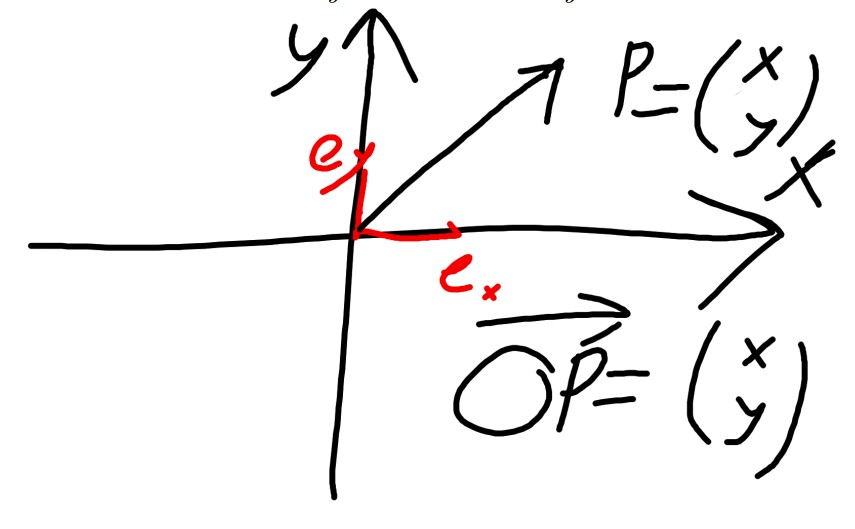
\includegraphics[scale=0.25]{imgs/22-01-24img01.jpg}\\
Den ortogonala projektionen av $\bm{v}$ på x-axeln ges av $x\bm{e}_{x}=\begin{pmatrix}x\\O\end{pmatrix}$.
\clearpage
\section{Koordinatsystem i ett rum}
Vi inför ett \underline{koordinatsystem i rummet} som följer.
\begin{enumerate}
    \item Vi fixerar en punkt O, origo
    \item Vi väljer tre enhetsvektorer $\bm{e}_{x},\bm{e}_{y}, \bm{e}_{z}$ som är parvis ortogonala.\\ 
        Vi skriver detta som $\bm{v}=\begin{pmatrix}x\\y\\z\end{pmatrix}$
    \item Vi kallar x,y,z för $\bm{v}$:s koordinater med avseende på basen $\bm{e}_{x}$, $\bm{e}_{y}$, $\bm{e}_{z}$.
\end{enumerate}
En bas $\bm{e}_{x}$, $\bm{e}_{y}$, $\bm{e}_{z}$ av enhetsvektorer och där vektorerna är parvis ortogonala kallas för en ON-bas (Orto Normal bas).\\
Om $\overrightarrow{OP}=\begin{pmatrix}x\\y\\z\end{pmatrix}$ så säger vi att punkten P har koordinaterna x,y,z,\\
alltså $\bm{v}=\bm{v}_{x} + \bm{v}_{y} + \bm{v}_{z} = x\bm{e}_{x} + y\bm{e}_{y} + z\bm{e}_{z}$\\
Vi väljer (nästan alltid) en ON-Bas så att ($\bm{e}_{x}$, $\bm{e}_{y}$, $\bm{e}_{z}$) är högerorienterad

\paragraph{Proposition 1.37} Följande regler gäller för koordinaterna av vektorer:
\begin{enumerate}
    \item $\begin{pmatrix}x_{1}\\y_{1}\\z_{1}\end{pmatrix}+\begin{pmatrix}x_{2}\\y_{2}\\z_{2}\end{pmatrix}=\begin{pmatrix}x_{1}+x_{2}\\y_{1}+y_{2}\\z_{1}+z_{2}\end{pmatrix}$
    \item $c\begin{pmatrix}x_{1}\\y_{1}\\z_{1}\end{pmatrix}=\begin{pmatrix}cx_{1}\\cy_{1}\\cz_{1}\end{pmatrix}$
\end{enumerate}

\paragraph{Sats 1.38} Om $\bm{u}=\begin{pmatrix}x_{1}\\y_{1}\\z_{1}\end{pmatrix}$ och $\bm{v}=\begin{pmatrix}x_{2}\\y_{2}\\z_{2}\end{pmatrix}$ i en ON-bas då är\\
\indent $\bm{u}\cdot \bm{v}=x_{1}x_{2}+y_{1}y_{2}+z_{1}z_{2}$\\
\indent $||\bm{u}||^{2}=x_{1}^2+y_{1}^{2}+z_{1}^{2}$
\subparagraph{Bevis} 
Låt $\bm{e}_{x}$, $\bm{e}_{y}$, $\bm{e}_{z}$ vara ON-basen.\\
Då är $||\bm{e}_{x}||= 1 =||\bm{e}_{y}||=||\bm{e}_{z}||$ och 
$\bm{e}_{x}\cdot \bm{e}_{y}=0=\bm{e}_{x}\cdot \bm{e}_{z}=\bm{e}_{y}\cdot \bm{e}_{z}$.\\
Vi har dessutom att
\begin{itemize}
    \item[] $\bm{u}=x_{1}\bm{e}_{x}+y_{1}\bm{e}_{y}+z_{1}\bm{e}_{y}+z_{1}\bm{e}_{z}$
    \item[] $\bm{v}=x_{2}\bm{e}_{x}+y_{2}\bm{e}_{y}+z_{2}\bm{e}_{y}+z_{2}\bm{e}_{z}$ 
\end{itemize}
$\bm{u}\cdot \bm{v} = (x_{1}\bm{e}_{x}+y_{1}\bm{e}_{y}+z_{1}\bm{e}_{y}+z_{1}\bm{e}_{z})\cdot (x_{2}\bm{e}_{x}+y_{2}\bm{e}_{y}+z_{2}\bm{e}_{y}+z_{2}\bm{e}_{z})=\\
=x_{1}x_{2}\bm{e}_{x}\cdot \bm{e}_{x}+y_{1}y_{2}\bm{e}_{y}\cdot \bm{e}_{y}+z_{1}z_{2}\bm{e}_{z}\cdot \bm{e}_{z}=x_{1}x_{2}||\bm{e}_{x}||^{2}+y_{1}y_{2}||\bm{e}_{y}||^{2}+z_{1}z_{2}||\bm{e}_{z}||^{2}=\\
=x_{1}x_{2}+y_{1}y_{2}+z_{1}z_{2}$ v.s.b

\clearpage
\paragraph{Ex} Beräkna vinkeln mellan $\bm{u}=\begin{pmatrix}2\\1\\3\end{pmatrix}$ och $\bm{v}=\begin{pmatrix}3\\4\\1\end{pmatrix}$.
\subparagraph{Lösning} Låt $\alpha$ vara vinkeln. Då är $\bm{u}\cdot \bm{v} = ||\bm{u}||\cdot ||\bm{v}||cos(\alpha)$\\
Vi vet att $\bm{u}\cdot \bm{v}=\begin{pmatrix}2\\1\\3\end{pmatrix}\cdot \begin{pmatrix}3\\4\\1\end{pmatrix}=2\cdot 3+1\cdot 4+3\cdot 1=6+4+3=13$
$||\bm{u}||=\sqrt{2^{2}+1^{2}+3^{2}}=\sqrt{4+1+9}=\sqrt{14}$
$||\bm{v}||=\sqrt{3^{2}+4^{2}+1^{2}}=\sqrt{9+16+1}=\sqrt{26}$
Alltså: $cos(\alpha)=\frac{\bm{u}\cdot \bm{v}}{||\bm{u}||\cdot ||\bm{v}||}=\frac{13}{\sqrt{4}\sqrt{26}}=\frac{13\sqrt{13}}{\sqrt{2}\sqrt{7}\sqrt{2}\sqrt{13}\sqrt{13}}=\frac{\sqrt{13}}{2\sqrt{7}}$
Därför är $\alpha=arccos(\frac{\sqrt{13}}{2\sqrt{7}})$.

\paragraph{Sats 1.42} Om $\bm{u}=\begin{pmatrix}x_{1}\\y_{1}\\z_{1}\end{pmatrix}$ och $\bm{v}=\begin{pmatrix}x_{2}\\y_{2}\\z_{2}\end{pmatrix}$ i en högerorienterad ON-bas då är 
\begin{equation*}
    \bm{u}\times \bm{v}=\begin{pmatrix}
        y_{1}z_{2}-z_{1}y_{2}\\
        z_{1}x_{2}-x_{1}z_{2}\\
        x_{1}y_{2}-y_{1}x_{2}
    \end{pmatrix}
\end{equation*}


\paragraph{Ex} Bestäm en vektor som är ortogonal mot både $\bm{u}=\begin{pmatrix}2\\3\\4\end{pmatrix}$ och $\bm{v}=\begin{pmatrix}2\\1\\5\end{pmatrix}$.
\subparagraph{Lösning} Vi vet att $\bm{u}\times \bm{v}$ är ortogonal mot $\bm{u}$ och $\bm{v}$!
\begin{equation*}
    \bm{u}\times \bm{v}=\begin{pmatrix}
        3\cdot 5-4\cdot 1\\
        4\cdot 2 - 2\cdot 5\\
        2\cdot 1 - 3\cdot 2
    \end{pmatrix} = 
    \begin{pmatrix}
        15-4\\
        9-16\\
        2-6
    \end{pmatrix} = \begin{pmatrix}11\\-2\\-4\end{pmatrix}
\end{equation*}

\chapter{Linjer och plan (Avs 1.6)}
\subsection{Linjer}
Samtliga linjer i planet går att beskriva med en ekvation på $Ax+By+C=0$.
Om $B\neq 0$ så är det samma sak som $By=-C-Ax \Leftrightarrow y=\frac{C}{B} - \frac{A}{B}x$ så typ $y=kx+m$

\begin{wrapfigure}{r}{0.6\textwidth}
    \vspace{-20pt}
    \centering
    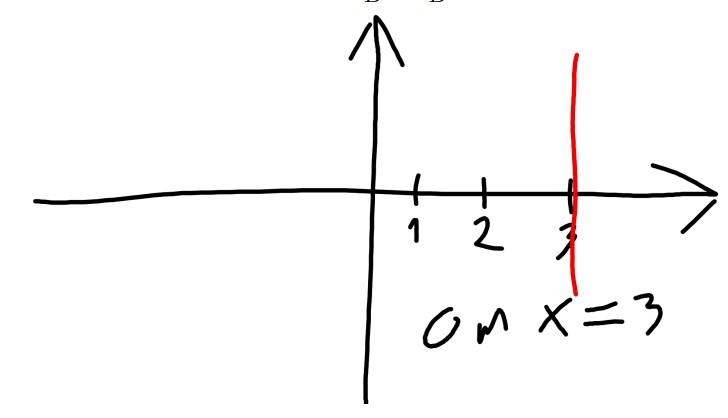
\includegraphics[scale=0.25]{imgs/22-01-24img02.jpg}\\
    \vspace{-30pt}
\end{wrapfigure}
\paragraph{Ex} Vad är $x=3$ för linje?\\
Här är $B=0$!\\
Värt att tillägga är att $y$-axeln beskrivs av ekvationen x=0.

\paragraph{Definition} En linje bestäms av en punkt $P_{0}$ och en riktningsvektor $\bm{v}$.
Samtliga punkter på linjen går att skriva som 
\begin{equation*}
    \begin{pmatrix}
        x\\y\\z
    \end{pmatrix}=
    \begin{pmatrix}
        x_{0}\\y_{0}\\z_{0}
    \end{pmatrix}+ \begin{pmatrix}
        v_{x}\\v_{y}\\v_{z}
    \end{pmatrix}=P_{0}+t\bm{v}\text{, }\forall t\in\mathbb{R}
\end{equation*}

